%%%%%%%%%%%%%%%%%%%%%%%%%%%%%%%%%%%%%%%%%
% Beamer Presentation
% LaTeX Template
% Version 1.0 (10/11/12)
%
% This template has been downloaded from:
% http://www.LaTeXTemplates.com
%
% License:
% CC BY-NC-SA 3.0 (http://creativecommons.org/licenses/by-nc-sa/3.0/)
%
%%%%%%%%%%%%%%%%%%%%%%%%%%%%%%%%%%%%%%%%%

%----------------------------------------------------------------------------------------
%	PACKAGES AND THEMES
%----------------------------------------------------------------------------------------

\documentclass{beamer}

\usepackage{booktabs}% http://ctan.org/pkg/booktabs
\newcommand{\tabitem}{~~\llap{\textbullet}~~}
%\usepackage{enumitem}
\usepackage{adjustbox}
\usepackage{anyfontsize}
%\usepackage{fontspec}

%\setmainfont{CMU Serif}

\mode<presentation> {

\usepackage{changepage}
%\usetheme{Warsaw}
\usetheme{Madrid}
%\setbeamertemplate{footline} % To remove the footer line in all slides uncomment this line
%\setbeamertemplate{footline}[page number] % To replace the footer line in all slides with a simple slide count uncomment this line

\setbeamertemplate{navigation symbols}{} % To remove the navigation symbols from the bottom of all slides uncomment this line
}

\usepackage{graphicx} % Allows including images
\usepackage{booktabs} % Allows the use of \toprule, \midrule and \bottomrule in tables

%----------------------------------------------------------------------------------------
%	TITLE PAGE
%----------------------------------------------------------------------------------------

\title[mpOTR]{Multi party Off-the-Record messaging protocol} % The short title appears at the bottom of every slide, the full title is only on the title page

\author{Andrikopoulos Konstantinos} % Your name
\institute[NTUA] % Your institution as it will appear on the bottom of every slide, may be shorthand to save space
{
National Technological University of Athens 
\includegraphics[scale=0.1]{Pyrforos.png} \\ % Your institution for the title page
\medskip
\textit{gkonstandinos@gmail.com} % Your email address
}
\date{Febuary 22, 2016} % Date, can be changed to a custom date


\begin{document}

\begin{frame}
\titlepage % Print the title page as the first slide
\end{frame}

\begin{frame}
\frametitle{Overview} % Table of contents slide, comment this block out to remove it
\tableofcontents % Throughout your presentation, if you choose to use \section{} and \subsection{} commands, these will automatically be printed on this slide as an overview of your presentation
\end{frame}

%----------------------------------------------------------------------------------------
%	PRESENTATION SLIDES
%----------------------------------------------------------------------------------------

%------------------------------------------------
\section{Multi party messaging challenges} % Sections can be created in order to organize your presentation into discrete blocks, all sections and subsections are automatically printed in the table of contents as an overview of the talk
%------------------------------------------------

\begin{frame}
OTR provides all we need in order to build Enrypted, Authenticated, Deniable and Forward secret connections between two peers.\\[0.2cm]

Why can't we simply extend plain OTR so that each user connects to every other party with OTR? This way we can have all the good stuff we get from OTR with virtually zero extra cost.\\[0.2cm]

This idea is not completely wrong. But it fails both for practical considerations and mainly because the naive extension is unable to provide basic properties that are crucial in multi party conversations
\end{frame}




\subsection{Practical considerations}
\begin{frame}
By building an otr connection for each peer we have to do the following. Encrypt and sign the message for every otr channel and maintain the data needed for each connection.\\[0.5cm]

This not only adds complexity to the protocol and implementation but also uses a lot of cpu time for each encryption and signing.
\end{frame}

\subsection{Theoretical considerations}
\begin{frame}
The main point is however that a multi party chat introduces challenges that are not present in a two peer conversation. For example:

\begin{itemize}
\item Ice cream attack
\item Messages consistency 
\item Room moderation
\end{itemize}
\end{frame}

\begin{frame}
It is clear that we need an approach that is multi-party oriented from the beggining and is not just a hack of an existing two party protocol.
\end{frame}

\begin{frame}
Some ideas for the practical challenges:

\begin{itemize}
\item Use a group key known to all members. One encryption operation needed!
\item Use public key signatures. One signing operation needed!

\end{itemize}
How ever we must keep in mind that we also need to preserve the OTR properties. For example public key signatures might not get along with deniability.
\end{frame}


\begin{frame}
Now for message consistency the original mpOTR paper "solves" the problem by hashing the set of messages received from each participant (for example in lexicographical ordering) and comparing the hashes between the parties.\\[0.5cm]

Note that this can only reveal if participants read the same messages, but not if they read them in the same order. Message reordering (ice cream attack) is not dealt with.
\end{frame}

\section{mpOTR from above}
\begin{frame}
So now lets see an overview of the mpOTR protocol.
\end{frame}

\begin{frame}
Before any cryptographical protocols are run the group participants must produce a session ID.  This is done by each user selecting a random number and broadcasting it to anyone else.\\[0.5cm]

Then the session ID is the hash of all participants and their random number contributions ordered lexicographically.\\[0.5cm]

Any messages sent now are unauthenticated and on the clear. When the group has produced an encrypting and a signing key table, the session ID will be authenticated too.
\end{frame}

\subsection{DSKE}
\begin{frame}
One of the most important steps in mpOTR is the eshtablishment of the keys used for the signing of the messages.\\[0.5cm]

Remember that we want to use public key crypto but remain deniable. The solution to this problem is to exchange public keys in a deniable but authenticated fashion!\\[0.5cm]
 
This way we will be able to authenticate messages sent from other chat participants but noone will be able to link messages we have signed to us, since the key exchange was deniable.
\end{frame}

\begin{frame}
\title{DSKE}
In mpOTR terms this is called a Deniable Secure Key exhange, or DSKE for short.\\[0.5cm]

Abstractly DSKE is an algorithm that, once executed by all members of the chat, will leave each member with an association table between the other participants and their AUTHENTICATED public keys, or it will fail if it was impossible to authenticate a participant.
\end{frame}

\begin{frame}
To do that it relies on the existance of an algorithm called Deniable Authenticated Key Exchange.\\[0.5cm]

This algorithm is run only between two chat participants. It takes as inputs the identities of those participants and creates deniably and securely an encrypting and a mac'ing key.\\[0.5cm]

With those keys some confirmation messages are sent to ensure that the two parites actually arrived at the same values. If the confirmation messages check out then each party is assured that the other participants public key really belongs to him.
\end{frame}

\begin{frame}
With a denAKE algorithm available DSKE uses it with every pair of pariticipants, with each user using the same public-private key pair for every run of the denAKE.\\[0.5cm]

The result for every user is an association table between chat participants and public keys.\\[0.5cm]

As a final step each user hashes his association table, signs the hash with the signing key, and sends the hash to everyone else. If the same hash is received from all other users then each paritcipant is assured that everyone has the same view of the chatroom members.
\end{frame}

\begin{frame}
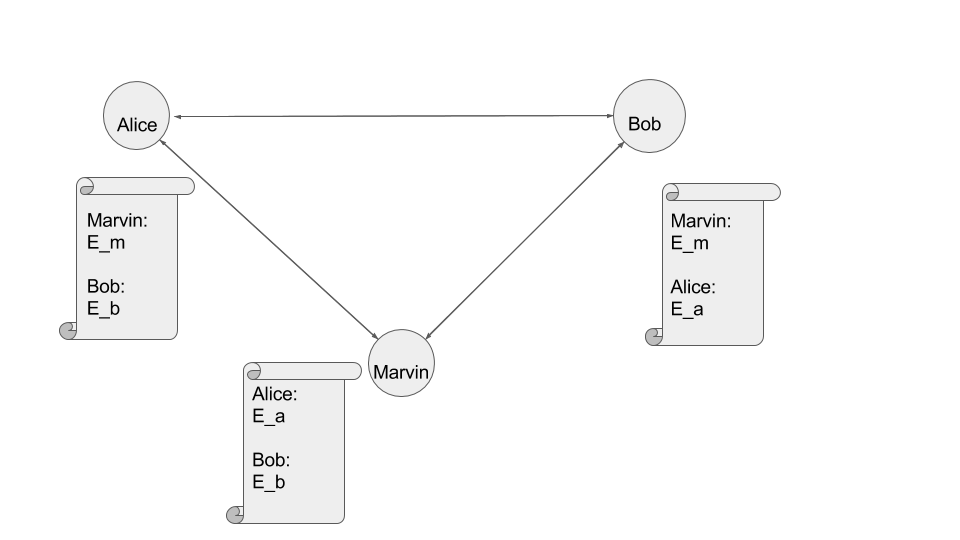
\includegraphics[scale=0.4]{denAKE.png}
\end{frame}


\subsection{GKA}

\begin{frame}
After each participant has formed his association table and compared it with everyone else's a group key is needed for encrypting the messages.\\[0.5cm]

Given the session ID and the association table a typical Group Key Agreement protocol can be executed in order to arrive at a group secret key $g_k$ for message encryption.\\[0.5cm]

GKAs are well studied so mpOTR paper does not spend to much time covering them.
\end{frame}

\begin{frame}
Note that since everything is deniable, subsequent signatures by any chat member are also, of course, deniable.\\[0.5cm]

Also a user can even deny participating in a given chatroom, something that otr does not provide since every time you start a conversation you sign some values with your private longterm key.\\[0.5cm]

This means that if every participant in a chatroom cooperates, it is possible to produce transcripts of the key exchange protocols so that any other users appears to have participated when in fact they a have not.
\end{frame}

\begin{frame}
With a signing key table and a group encryption key the participants can authenticate the session ID and any other protocol parameters that they may have negotiated before they could authenticate them (for example protocol version).\\[0.5cm]

This is done by hashing the session ID and any other parameters, then encrypting and signing the hash with the keys created in DSKE and GKA and broadcasting the result. Each user then checks if he received the same hash from all other users.
\end{frame}

\subsection{Communicating}

\begin{frame}
The communication phase in mpOTR is trivial.\\[0.5cm]

For encryption it uses a symmetric algorithm with $g_k$ being the encryption key derived from the GKA.\\[0.5cm]

This algorithm needs to be secure under a chosen plaintext attack.
\end{frame}

\begin{frame}
For signing messages a public key, existentially unforgeable, signature scheme is used, with each user signing with the key that was authenticated during the DSKE.\\[0.5cm]


\end{frame}

\begin{frame}
To send a message a user first encrypts the data, producing the ciphertext $C$, while storing the plaintext in the \emph{sent} message list.\\[0.5cm]

Then he signs the session ID $sid$ concatenated with $C$, producing the signature $\sigma$.\\[0.5cm]

Finally he broadcasts the message $\langle sid, C, \sigma \rangle$.
\end{frame}

\begin{frame}
Upon receiving a message a user needs to make sure that it is signed correctly and also that it is intended for the chatroom in question, by checking $sid$. The plaintext message is also stored in the \emph{received} chat's message list that corresponds to the author of the message.\\[0.5cm]

Note that an attacker cannot alter a message or inject his own messages but is able to drop or duplicate a message. In mpOTR's case this is tackled at the end of the conversation in the shutdown phase.\\[0.5cm]

A dishonest participant is also able to send one message to user $A$ and another to user $B$.
\end{frame}


\subsection{Shutdown phase}
\begin{frame}
The shutdown phase is initiated when both of these hold true:

\begin{itemize}
\item[A] The user has requested for the conversation to end, and
\item[B] there are no messages in-flight between the users.
\end{itemize}
\end{frame}

\begin{frame}
To establish that there is a consensus over the set of the messages, each participant $X$ hashes his \emph{sent} list (ordered lexixographically), producing the hash $h_x$ and broadcasts the tuple $\langle "shutdown", h_x \rangle$.\\[0.5cm]

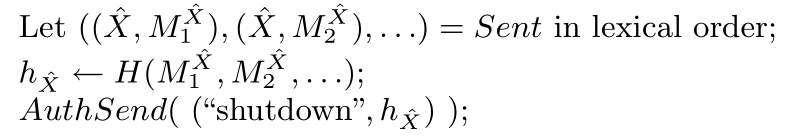
\includegraphics[scale=0.4]{sent_hash.png}
\end{frame}

\begin{frame}
After that he will patiently wait to receive the shutdown message from all the other participants.\\[0.5cm]

When he receives a shutdown message from user $Y$ he shall, store the hash this message contains, then hash on his own this users \emph{received} list  and finally mark that he is no longer waiting messages from user $Y$.\\[0.5cm]

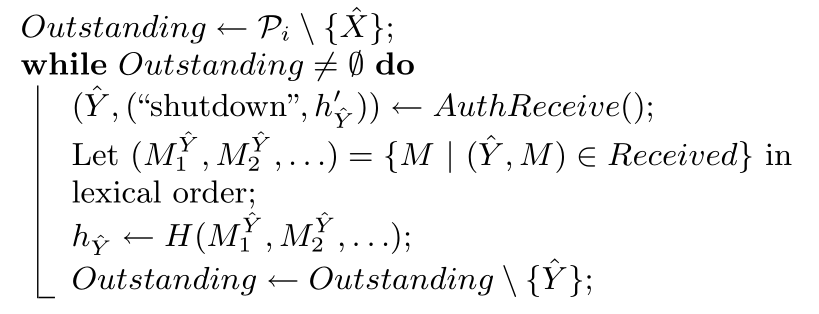
\includegraphics[scale=0.4]{received_hashes.png}
\end{frame}

\begin{frame}
After he has received the shutdown messages from all users he will hash his \emph{sent} hash with all the received hashes together, producing a digest $h$ of the whole chat, and broadcasts the tuple $\langle "digest", h$.\\[0.5cm]

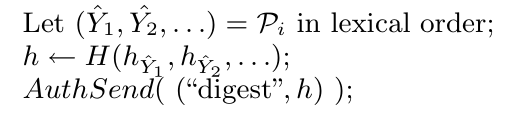
\includegraphics[scale=0.4]{chat_digest.png}
\end{frame}

\begin{frame}
He will again wait to receive the digest messages from all other users and compare the received digests with the one he produced earlier in order to determine if a consensus is reached.\\[0.5cm]

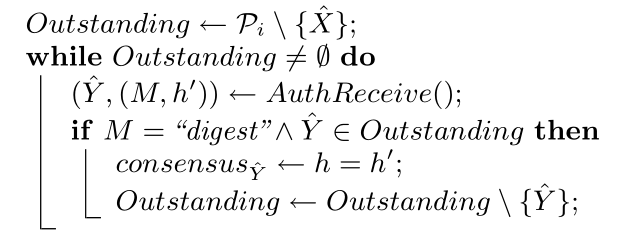
\includegraphics[scale=0.4]{determine_consensus.png}
\end{frame}

\begin{frame}
After that he informs the other users that he does not intend to send any messages, and waits to receive such confirmations from the rest of the users.\\[0.5cm]

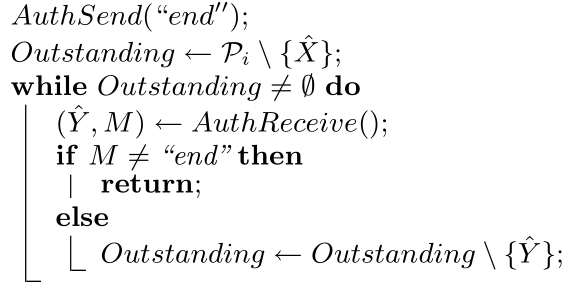
\includegraphics[scale=0.4]{no_listen_verify.png}\\[1cm]

And finally he broadcasts his signing key.
\end{frame}
\end{document} 